\begin{table}[b]
    \centering
    \begin{tabular}{llc}
        \hline
        \textbf{Parameter} & \textbf{Description} & \textbf{Type} \\
        \hline
        \multicolumn{3}{c}{\textbf{Single-Qubit Gate Parameters (7)}} \\
        $k_{\text{dep}}$ & Depolarizing scaling factor & Stochastic \\
        $b_{\text{dep}}$ & Depolarizing offset & Stochastic \\
        $b_{\text{amp}}$ & Amplitude damping offset & Stochastic \\
        $\theta_{x,y,z}$ & Coherent rotation angles & Coherent \\
        $\beta_{1\text{Q}}$ & Stretched dephasing exponent & Non-Markovian \\
        \hline
        \multicolumn{3}{c}{\textbf{Two-Qubit Gate Parameters (9)}} \\
        $k_{\text{dep,2Q}}$ & Depolarizing scaling factor & Stochastic \\
        $b_{\text{dep,2Q}}$ & Depolarizing offset & Stochastic \\
        $b_{\text{amp,2Q}}$ & Amplitude damping offset & Stochastic \\
        $b_{\phi,2Q}$ & Phase damping offset & Stochastic \\
        $\theta_{\text{ixx,yy,zz}}$ & Coherent crosstalk angles & Coherent \\
        $\beta_{2\text{Q}}$ & Stretched dephasing exponent & Non-Markovian \\
        $k_{zz}$ & Correlated ZZ dephasing rate & Correlated \\
        \hline
        \multicolumn{3}{c}{\textbf{Correlated Readout Parameters (4)}} \\
        $a, b_{00\leftrightarrow 11}$ & Coefficients (\textbar 00 \textgreater \(\leftrightarrow\) \textbar 11 \textgreater) & Correlated \\
        $a, b_{01\leftrightarrow 10}$ & Coefficients (\textbar 01 \textgreater \(\leftrightarrow\) \textbar 10 \textgreater) & Correlated \\
        \hline
    \end{tabular}
    \caption{Gate and readout parameters as described in \cite{ji_data-efficient_2025}}
    \label{tab:jiparameters}
\end{table}

\begin{figure}
    \centering
    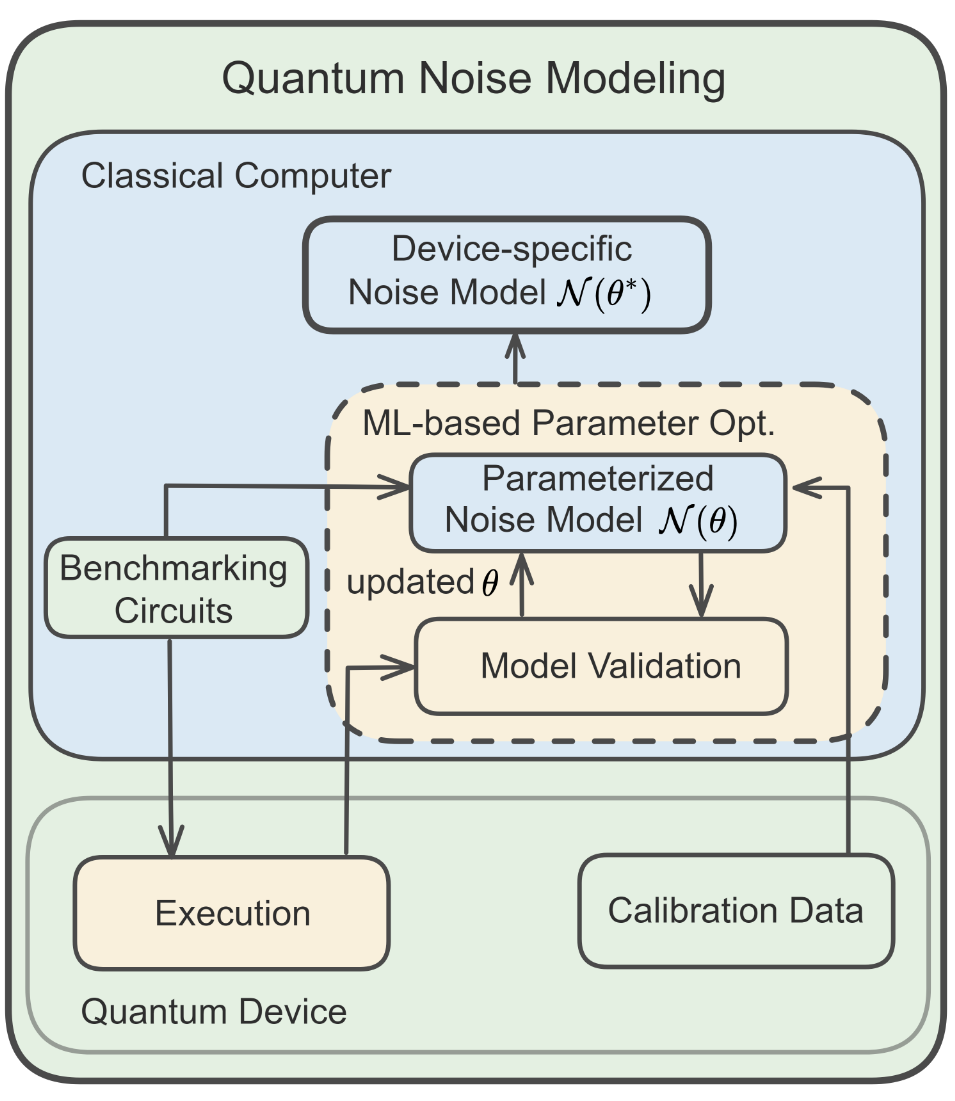
\includegraphics[width=0.5\linewidth]{figures/jie_framework.png}
    \caption{Framework outline for noise modeling in section \ref{sec:jiModeling}}
    \label{fig:ji_framework}
\end{figure}